\section{Indici basati su Hash}

Gli indici basati su hash mappano una chiave di ricerca direttamente all'identificatore di pagina (pid) della pagina (o catena di overflow) che la contiene.

\textbf{Caratteristiche principali:}
\begin{itemize}
    \item \textbf{Ottimi per ricerche di uguaglianza (equality search):} Es. \texttt{WHERE nome = 'Mario'}.
    \item \textbf{Non efficienti per ricerche su intervalli (range search):} Es. \texttt{WHERE eta > 30}.
    \item Usano \textbf{blocchi} per memorizzare i \textbf{bucket}.
\end{itemize}

Esistono due macro-categorie:
\begin{enumerate}
    \item \textbf{Hashing Statico:} Per dati di dimensione fissa e non modificabili (es. CD-ROM).
    \item \textbf{Hashing Dinamico (Estensibile e Lineare):} Quando dati e dimensioni dei dati possono variare nel tempo.
\end{enumerate}

\subsection{Hashing Statico}

L'hashing statico utilizza un numero fisso $N$ di bucket e una funzione di hash $H$ che mappa la chiave di ricerca in un intervallo da 0 a $N-1$.
Negli esempi, useremo funzioni di hash $H_i$ che restituiscono i primi (o gli ultimi) $i$ bit della codifica binaria della chiave.

\textbf{Esempio Base:}
\begin{itemize}
    \item $i = 1$ (si usa il primo bit più significativo).
    \item $N = 2^i = 2^1 = 2$ bucket (bucket 0 e bucket 1).
    \item Ogni bucket contiene un blocco.
    \item Chiavi (già codificate in binario): \texttt{0001}, \texttt{1001}, \texttt{1100}.
    \begin{itemize}
        \item $H_1(\texttt{0001})$ $\rightarrow$ primo bit è \texttt{0} $\rightarrow$ bucket 0.
        \item $H_1(\texttt{1001})$ $\rightarrow$ primo bit è \texttt{1} $\rightarrow$ bucket 1.
        \item $H_1(\texttt{1100})$ $\rightarrow$ primo bit è \texttt{1} $\rightarrow$ bucket 1.
    \end{itemize}
\end{itemize}

Struttura risultante:
\begin{itemize}
    \item Bucket 0: [\texttt{0001}]
    \item Bucket 1: [\texttt{1001}, \texttt{1100}]
\end{itemize}

\begin{figure}[h]
\centering
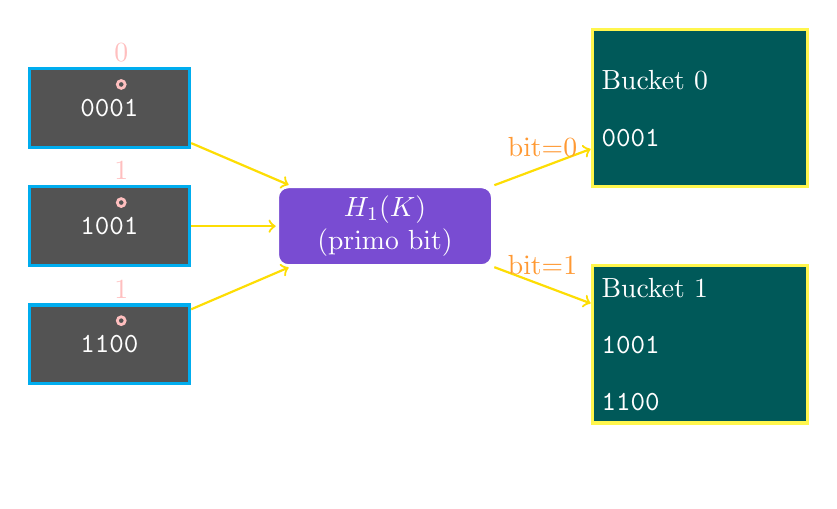
\begin{tikzpicture}[node distance=2.5cm]
    % Stile per i nodi
    \tikzstyle{key}=[rectangle, draw, fill=darkgray!90, text=white, text width=1.8cm, text centered, minimum height=1cm, node distance=3cm, line width=1.2pt, draw=cyan]
    \tikzstyle{hash}=[rectangle, draw, fill=violet!50!blue!70, text=white, text width=2.5cm, text centered, rounded corners, minimum height=1cm, line width=1.2pt, draw=white]
    \tikzstyle{bucket}=[rectangle, draw, fill=teal!70!black, text=white, text width=2.5cm, minimum height=2cm, node distance=4cm, line width=1.2pt, draw=yellow!70]
    \tikzstyle{overflow}=[rectangle, draw, fill=orange!50!black, text=white, text width=2.5cm, minimum height=1.5cm, node distance=4cm, line width=1.2pt, draw=yellow!70, dashed]
    \tikzstyle{arrow}=[->, thick, yellow!80!orange]
    \tikzstyle{overflow_arrow}=[->, thick, orange!90, dashed]
    
    % Chiavi di input
    \node[key] (key1) at (0,0) {\texttt{0001}};
    \node[key] (key2) at (0,-1.5) {\texttt{1001}};
    \node[key] (key3) at (0,-3) {\texttt{1100}};
    
    % Funzione hash
    \node[hash] (hash) at (3.5,-1.5) {$H_1(K)$\\(primo bit)};
    
    % Bucket
    \node[bucket] (bucket0) at (7.5,0) {Bucket 0\\[0.3cm]\texttt{0001}};
    \node[bucket] (bucket1) at (7.5,-3) {Bucket 1\\[0.3cm]\texttt{1001}\\[0.3cm]\texttt{1100}};
    
    % Etichette dei bucket
    \node[text=white] at (7.5,-4.5) {$N = 2$ bucket};
    
    % Frecce dalle chiavi alla funzione hash
    \draw[arrow] (key1) -- (hash);
    \draw[arrow] (key2) -- (hash);
    \draw[arrow] (key3) -- (hash);
    
    % Frecce dalla funzione hash ai bucket
    \draw[arrow] (hash) -- node[above, text=orange!80] {bit=0} (bucket0);
    \draw[arrow] (hash) -- node[above, text=orange!80] {bit=1} (bucket1);
    
    % Annotazioni per evidenziare il primo bit
    \node[draw, circle, pink, inner sep=1pt, line width=1pt] at (0.15,0.3) {};
    \node[pink] at (0.15,0.7) {0};
    
    \node[draw, circle, pink, inner sep=1pt, line width=1pt] at (0.15,-1.2) {};
    \node[pink] at (0.15,-0.8) {1};
    
    \node[draw, circle, pink, inner sep=1pt, line width=1pt] at (0.15,-2.7) {};
    \node[pink] at (0.15,-2.3) {1};
\end{tikzpicture}
\caption{Visualizzazione dell'hashing statico con $H_1$ (primo bit)}
\end{figure}

\subsubsection{Ricerca (Searching)}
Si calcola l'hash della chiave data per trovare il bucket e si cerca il record all'interno di quel bucket (e delle sue eventuali catene di overflow).

\textbf{Esempio:}
\begin{itemize}
    \item Cercare $K = \texttt{1100}$.
    \item Funzione Hash: $H_1$ (usa il primo bit).
    \item $H_1(\texttt{1100})$ $\rightarrow$ il primo bit è \texttt{1}.
    \item Si accede al bucket \texttt{1}.
    \item Si scorre il blocco (o i blocchi) del bucket \texttt{1} fino a trovare (o non trovare) \texttt{1100}.
\end{itemize}

\subsubsection{Inserimento (Insertion)}
L'hashing statico non può cambiare il numero di bucket. Se un bucket è pieno, si usa una \textbf{catena di blocchi di overflow}.

\textbf{Esempio:}
\begin{itemize}
    \item Stato attuale come sopra. Inserire $K = \texttt{1010}$.
    \item Funzione Hash: $H_1$.
    \item $H_1(\texttt{1010})$ $\rightarrow$ il primo bit è \texttt{1}.
    \item Si accede al bucket \texttt{1}.
    \item Supponiamo che il blocco primario del bucket \texttt{1} sia pieno (contenente \texttt{1001}, \texttt{1100}).
    \item Si crea un blocco di overflow collegato al blocco primario del bucket \texttt{1} e vi si inserisce \texttt{1010}.
\end{itemize}
Struttura dopo inserimento di \texttt{1010}:
\begin{itemize}
    \item Bucket 0: [\texttt{0001}]
    \item Bucket 1: [\texttt{1001}, \texttt{1100}] $\rightarrow$ [\texttt{1010}] (overflow)
\end{itemize}

\begin{figure}[h]
\centering
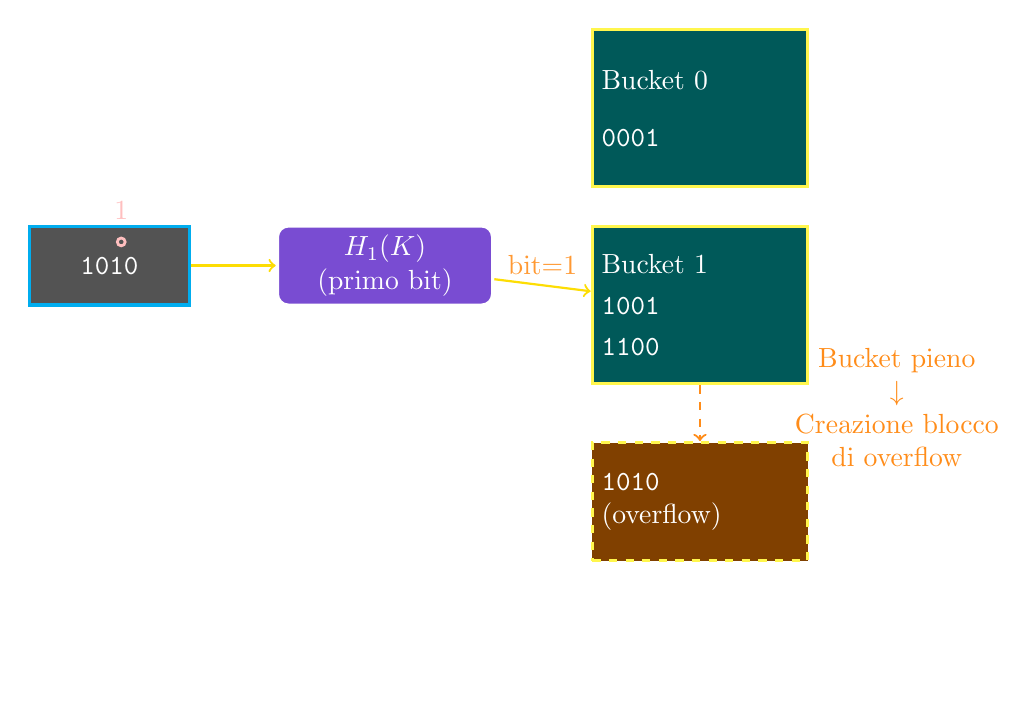
\begin{tikzpicture}[node distance=2.5cm]
    % Stile per i nodi
    \tikzstyle{key}=[rectangle, draw, fill=darkgray!90, text=white, text width=1.8cm, text centered, minimum height=1cm, node distance=3cm, line width=1.2pt, draw=cyan]
    \tikzstyle{hash}=[rectangle, draw, fill=violet!50!blue!70, text=white, text width=2.5cm, text centered, rounded corners, minimum height=1cm, line width=1.2pt, draw=white]
    \tikzstyle{bucket}=[rectangle, draw, fill=teal!70!black, text=white, text width=2.5cm, minimum height=2cm, node distance=4cm, line width=1.2pt, draw=yellow!70]
    \tikzstyle{overflow}=[rectangle, draw, fill=orange!50!black, text=white, text width=2.5cm, minimum height=1.5cm, node distance=4cm, line width=1.2pt, draw=yellow!70, dashed]
    \tikzstyle{arrow}=[->, thick, yellow!80!orange]
    \tikzstyle{overflow_arrow}=[->, thick, orange!90, dashed]
    
    % Chiave di input nuova
    \node[key] (key4) at (0,0) {\texttt{1010}};
    
    % Funzione hash
    \node[hash] (hash) at (3.5,0) {$H_1(K)$\\(primo bit)};
    
    % Bucket
    \node[bucket] (bucket0) at (7.5,2) {Bucket 0\\[0.3cm]\texttt{0001}};
    \node[bucket] (bucket1) at (7.5,-0.5) {Bucket 1\\[0.1cm]\texttt{1001}\\[0.1cm]\texttt{1100}};
    \node[overflow] (overflow) at (7.5,-3) {\texttt{1010}\\(overflow)};
    
    % Etichette
    \node[text=white] at (7.5,-4.5) {$N = 2$ bucket (fisso)};
    \node[text=white] at (7.5,-5) {3 blocchi totali};
    
    % Frecce
    \draw[arrow] (key4) -- (hash);
    \draw[arrow] (hash) -- node[above, text=orange!80] {bit=1} (bucket1);
    \draw[overflow_arrow] (bucket1) -- (overflow);
    
    % Annotazione per evidenziare il primo bit
    \node[draw, circle, pink, inner sep=1pt, line width=1pt] at (0.15,0.3) {};
    \node[pink] at (0.15,0.7) {1};
    
    % Annotazione per spiegare l'overflow
    \node[text=orange!90, align=center] at (10,-1.8) {Bucket pieno\\$\downarrow$\\Creazione blocco\\di overflow};
\end{tikzpicture}
\caption{Inserimento con overflow nell'hashing statico: il bucket 1 è pieno, quindi \texttt{1010} viene inserito in un blocco di overflow}
\end{figure}

\textbf{Domande Tipiche:}
Data la struttura risultante dall'inserimento di \texttt{1010}:
\begin{itemize}
    \item \textbf{Quanti bucket ci sono?} Ci sono \textbf{2} bucket (bucket 0 e bucket 1). Il numero di bucket è fisso.
    \item \textbf{Quanti blocchi ci sono?}
    \begin{itemize}
        \item Bucket 0: 1 blocco.
        \item Bucket 1: 1 blocco primario + 1 blocco di overflow.
        \item Totale: \textbf{3} blocchi.
    \end{itemize}
\end{itemize}

\subsubsection{Cancellazione (Deletion)}
Si individua il record e lo si rimuove. Se la rimozione svuota un blocco di overflow, questo può essere deallocato. Lunghe catene di overflow degradano le performance.

\textbf{Esempio:}
\begin{itemize}
    \item Stato attuale: Bucket 0: [\texttt{0001}]; Bucket 1: [\texttt{1001}, \texttt{1100}] $\rightarrow$ [\texttt{1010}].
    \item Cancellare $K = \texttt{1100}$.
    \begin{enumerate}
        \item $H_1(\texttt{1100})$ $\rightarrow$ bucket \texttt{1}.
        \item Si cerca \texttt{1100} nel bucket \texttt{1} e lo si rimuove dal suo blocco (il blocco primario).
    \end{enumerate}
    \item Se successivamente si cancellasse $K = \texttt{1010}$:
    \begin{enumerate}
        \item $H_1(\texttt{1010})$ $\rightarrow$ bucket \texttt{1}.
        \item Si cerca \texttt{1010} nel bucket \texttt{1}, trovandolo nel blocco di overflow.
        \item Si rimuove \texttt{1010}. Se il blocco di overflow diventa vuoto, può essere deallocato e il puntatore dal blocco primario rimosso.
    \end{enumerate}
\end{itemize}

\subsubsection{Efficienza dell'Hashing Statico}
\begin{itemize}
    \item \textbf{Ideale:} Lookup con un solo accesso al disco se il bucket sta in un blocco e non ci sono overflow.
    \item \textbf{Problema:} Lunghe catene di overflow degradano rapidamente le prestazioni (un accesso al disco per blocco).
    \item L'efficienza dipende da:
    \begin{itemize}
        \item Rapporto tra dimensione dell'indice e dati (numero di bucket).
        \item Distribuzione delle chiavi rispetto alla funzione hash.
    \end{itemize}
\end{itemize}
Per mitigare i problemi di overflow, si usano tecniche di hashing dinamico come l'hashing estensibile o lineare.

\subsection{Hashing Estensibile (Extendible Hashing)}
Introduce un livello di indirezione: una \textbf{directory di puntatori} ai blocchi.

\textbf{Caratteristiche principali:}
\begin{itemize}
    \item La directory dei puntatori può crescere; la sua lunghezza è sempre una potenza di 2.
    \item Raddoppiando la directory, raddoppia il numero di "bucket" (entry nella directory).
    \item Non è necessario un blocco dati per ogni bucket della directory; più bucket possono condividere un blocco.
    \item \textbf{Non usa blocchi di overflow.}
    \item La funzione hash $H_i$ restituisce i primi $i$ bit più significativi. $i$ è la \textbf{profondità globale} della directory.
    \item Ogni blocco ha una variabile $j$ (chiamata \textbf{profondità locale}) che indica quanti bit sono stati usati per l'indicizzazione \textit{di quel blocco}.
\end{itemize}

\textbf{Terminologia:}
\begin{itemize}
    \item $i$: profondità globale (numero di bit usati per indirizzare la directory). Dimensione directory = $2^i$.
    \item $j$: profondità locale (numero di bit usati per discriminare i record \textit{all'interno} di un blocco specifico). $j \le i$.
\end{itemize}

\subsubsection{Ricerca}
\begin{enumerate}
    \item Calcola $H_i(K)$ (primi $i$ bit della chiave K).
    \item Usa questo valore come indice nella directory per trovare il puntatore al blocco corretto.
    \item Accedi al blocco e cerca K.
\end{enumerate}

\textbf{Esempio:}
\begin{itemize}
    \item $i = 1$ (profondità globale). Directory ha $2^1 = 2$ entry (\texttt{0} e \texttt{1}).
    \item Blocco A (per chiavi che iniziano con \texttt{0...}): contiene \texttt{0001}. Profondità locale $j_A = 1$.
    \item Blocco B (per chiavi che iniziano con \texttt{1...}): contiene \texttt{1001}, \texttt{1100}. Profondità locale $j_B = 1$.
    \item Directory:
    \begin{itemize}
        \item \texttt{0} $\rightarrow$ Blocco A
        \item \texttt{1} $\rightarrow$ Blocco B
    \end{itemize}
    \item Cercare $K = \texttt{1100}$:
    \begin{enumerate}
        \item $H_1(\texttt{1100})$ (primo bit) $\rightarrow$ \texttt{1}.
        \item Directory[\texttt{1}] punta al Blocco B.
        \item Cerca \texttt{1100} nel Blocco B. Trovato.
    \end{enumerate}
\end{itemize}

\subsubsection{Inserimento (Insertion Steps)}
\begin{enumerate}
    \item \textbf{Trova il blocco:} Usa i primi $i$ bit della chiave $K$ ($H_i(K)$) per trovare l'entry nella directory e quindi il blocco $B$.
    \item \textbf{Se c'è spazio nel blocco B:} Inserisci il record. Fatto.
    \item \textbf{Se non c'è spazio nel blocco B:} Controlla la profondità locale $j$ del blocco $B$.
    \begin{itemize}
        \item \textbf{Caso A: $j < i$} (Il blocco B è condiviso da più entry della directory che differiscono solo dopo il $j$-esimo bit)
        \begin{enumerate}
            \item \textbf{Split del blocco B:} Crea un nuovo blocco $B'$.
            \item \textbf{Incrementa $j$:} La profondità locale di $B$ e $B'$ diventa $j+1$.
            \item \textbf{Distribuisci i record:} Riassegna i record del vecchio $B$ (più il nuovo record da inserire) tra $B$ e $B'$ basandoti sul valore del loro $(j+1)$-esimo bit.
            \item \textbf{Aggiorna la directory:} Alcune entry della directory che prima puntavano a $B$ ora punteranno a $B'$. In particolare, quelle entry che corrispondono ai record finiti in $B'$ (cioè quelle il cui prefisso di $i$ bit, quando si considerano $j+1$ bit, matcha i record in $B'$).
        \end{enumerate}
        \item \textbf{Caso B: $j == i$} (Il blocco B è "pieno" rispetto alla capacità discriminante della directory attuale)
        \begin{enumerate}
            \item \textbf{Incrementa $i$:} La profondità globale della directory diventa $i+1$.
            \item \textbf{Raddoppia la directory:} Ogni vecchia entry $w$ (lunga $i$ bit) nella directory genera due nuove entry $w0$ e $w1$ (lunghe $i+1$ bit). Inizialmente, entrambe puntano al blocco a cui puntava $w$.
            \item \textbf{Ora $j < i$ (nuovo $i$):} Procedi come nel Caso A per splittare il blocco B (la cui profondità locale $j$ è ora minore del nuovo $i$). La $j$ dei due blocchi risultanti diventerà $j_{\text{vecchio}}+1$.
        \end{enumerate}
    \end{itemize}
\end{enumerate}

\textbf{Esempio Inserimento (inserire \texttt{1010})}

\begin{figure}[h]
\centering
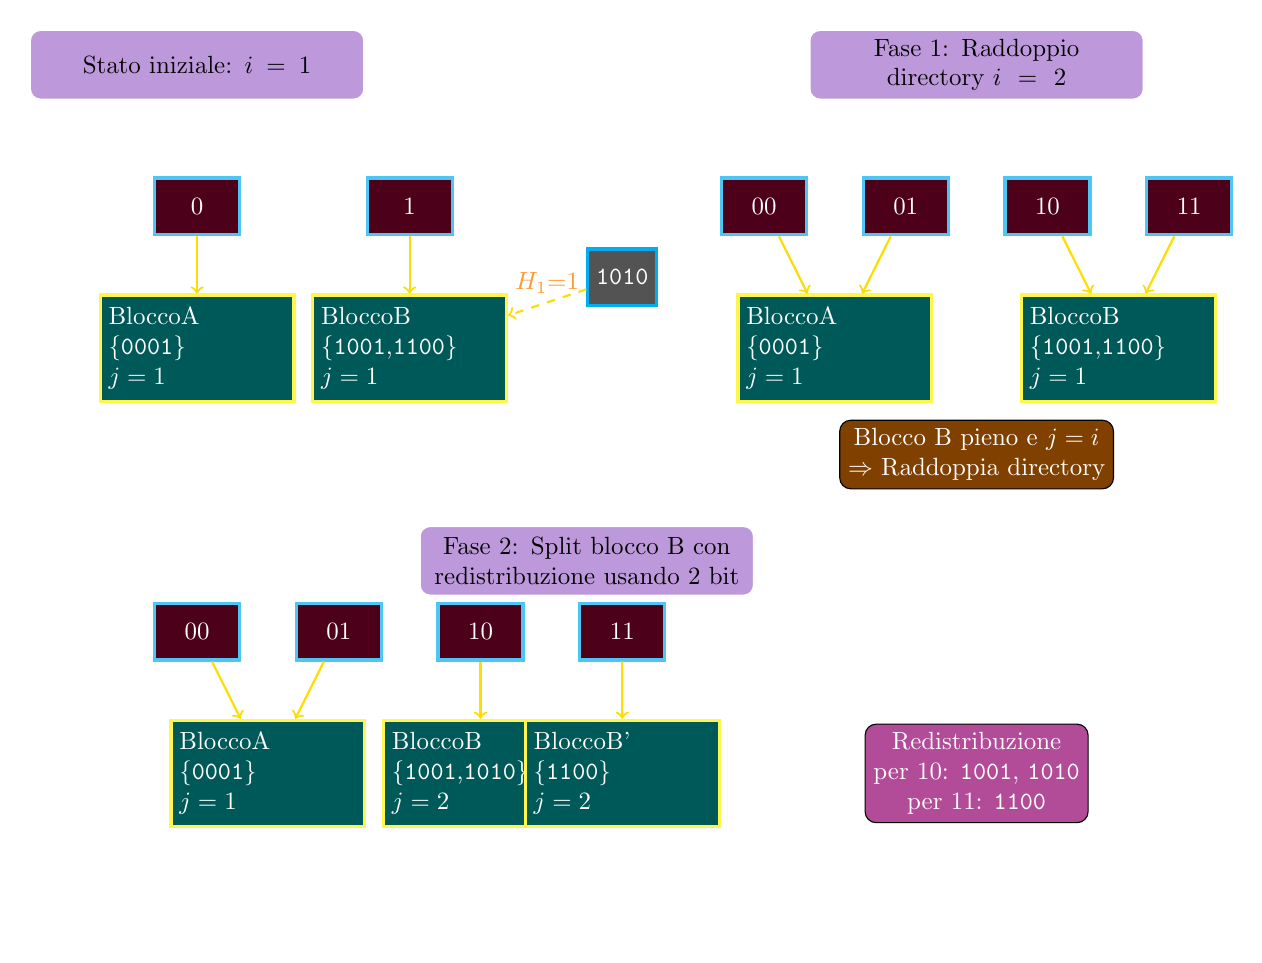
\begin{tikzpicture}[node distance=2.5cm, scale=0.9, transform shape]
    % Stili per i nodi
    \tikzstyle{directory}=[rectangle, draw, fill=purple!40!black, text=white, minimum width=1.2cm, minimum height=0.8cm, line width=1.2pt, draw=cyan!70]
    \tikzstyle{block}=[rectangle, draw, fill=teal!70!black, text=white, text width=2.5cm, minimum height=1.5cm, line width=1.2pt, draw=yellow!70]
    \tikzstyle{arrow}=[->, thick, yellow!80!orange]
    \tikzstyle{stepbox}=[rectangle, draw, fill=violet!70!blue!40, text=black, text width=4.5cm, text centered, rounded corners, minimum height=1cm, line width=1.2pt, draw=white]
    % Prima fase - Stato iniziale
    \node[stepbox] at (0,8) {Stato iniziale: $i=1$};
    
    \node[directory] (dir0) at (0,6) {0};
    \node[directory] (dir1) at (3,6) {1};
    \node[block] (blockA1) at (0,4) {BloccoA\\$\{$\texttt{0001}$\}$\\$j=1$};
    \node[block] (blockB1) at (3,4) {BloccoB\\$\{$\texttt{1001},\texttt{1100}$\}$\\$j=1$};
    
    \draw[arrow] (dir0) -- (blockA1);
    \draw[arrow] (dir1) -- (blockB1);
    
    % Nuova chiave da inserire
    \node[rectangle, draw, fill=darkgray!90, text=white, text centered, minimum height=0.8cm, line width=1.2pt, draw=cyan] (key) at (6,5) {\texttt{1010}};
    \draw[arrow, dashed] (key) -- node[above, text=orange!80] {$H_1$=1} (blockB1);
    
    % Seconda fase - Raddoppio directory
    \node[stepbox] at (11,8) {Fase 1: Raddoppio directory $i=2$};
    
    \node[directory] (dir00) at (8,6) {00};
    \node[directory] (dir01) at (10,6) {01};
    \node[directory] (dir10) at (12,6) {10};
    \node[directory] (dir11) at (14,6) {11};
    
    \node[block] (blockA2) at (9,4) {BloccoA\\$\{$\texttt{0001}$\}$\\$j=1$};
    \node[block] (blockB2) at (13,4) {BloccoB\\$\{$\texttt{1001},\texttt{1100}$\}$\\$j=1$};
    
    \draw[arrow] (dir00) -- (blockA2);
    \draw[arrow] (dir01) -- (blockA2);
    \draw[arrow] (dir10) -- (blockB2);
    \draw[arrow] (dir11) -- (blockB2);
    
    \node[draw, fill=orange!50!black, text=white, align=center, rounded corners] at (11,2.5) {Blocco B pieno e $j=i$\\$\Rightarrow$ Raddoppia directory};
    % Terza fase - Split blocco
    \node[stepbox] at (5.5,1) {Fase 2: Split blocco B con redistribuzione usando 2 bit};
    
    \node[directory] (dir00f) at (0,0) {00};
    \node[directory] (dir01f) at (2,0) {01};
    \node[directory] (dir10f) at (4,0) {10};
    \node[directory] (dir11f) at (6,0) {11};
    
    \node[block] (blockAf) at (1,-2) {BloccoA\\$\{$\texttt{0001}$\}$\\$j=1$};
    \node[block] (blockBf) at (4,-2) {BloccoB\\$\{$\texttt{1001},\texttt{1010}$\}$\\$j=2$};
    \node[block] (blockBpf) at (6,-2) {BloccoB'\\$\{$\texttt{1100}$\}$\\$j=2$};
    
    \draw[arrow] (dir00f) -- (blockAf);
    \draw[arrow] (dir01f) -- (blockAf);
    \draw[arrow] (dir10f) -- (blockBf);
    \draw[arrow] (dir11f) -- (blockBpf);
    
    % Redistribuzione
    \node[draw, fill=pink!40!violet, text=white, align=center, rounded corners] at (11,-2) {Redistribuzione\\per 10: \texttt{1001}, \texttt{1010}\\per 11: \texttt{1100}};
    
    % Annotazioni finali
    \node[text=white, align=center] at (5.5,-4) {Stato finale: $i=2$, 4 entry nella directory, 3 blocchi distinti};
\end{tikzpicture}
\caption{Visualizzazione dell'inserimento di \texttt{1010} nell'hashing estensibile}
\end{figure}

\textbf{Domande Tipiche:}
\begin{itemize}
    \item $i = 3$.
    \item Directory: \texttt{000, 001, 010, 011, 100, 101, 110, 111}.
    \item \textbf{Quanti bucket (entry della directory) ci sono?} $2^i = 2^3 =$ \textbf{8}.
    \item \textbf{Quanti blocchi ci sono?} Si contano i blocchi distinti puntati dalla directory (esempio):
    \begin{enumerate}
        \item \texttt{Blocco\_X (contiene 0001, j=2)} puntato da \texttt{000} e \texttt{001}.
        \item \texttt{Blocco\_Y (contiene 0100, 0101, j=2)} puntato da \texttt{010} e \texttt{011}.
        \item \texttt{Blocco\_Z (contiene 1001, 1000, j=3)} puntato da \texttt{100}.
        \item \texttt{Blocco\_W (contiene 1010, j=3)} puntato da \texttt{101}.
        \item \texttt{Blocco\_K (contiene 1100, j=2)} puntato da \texttt{110} e \texttt{111}.
    \end{enumerate}
    Totale: \textbf{5} blocchi distinti (in questo esempio).
\end{itemize}

\subsubsection{Osservazioni sull'Hashing Estensibile}
\begin{itemize}
    \item \textbf{Ricerca veloce:} Un solo accesso al disco se la directory è in memoria principale.
    \item \textbf{Split localizzati:} Solo i record di un blocco vengono ridistribuiti.
    \item \textbf{Svantaggi:}
    \begin{itemize}
        \item Se la ridistribuzione dopo uno split è sfortunata (es. tutti i record hanno gli stessi primi $j+1$ bit), potrebbe essere necessario splittare di nuovo subito.
        \item La directory cresce a scatti (raddoppia). Con distribuzioni di chiavi sbilanciate, la directory può diventare inutilmente grande.
        \item La crescita esponenziale della directory può complicarne la gestione e la memorizzazione in memoria principale.
    \end{itemize}
\end{itemize}

\subsection{Hashing Lineare}
Evita la necessità di una directory, ma gestisce il problema delle lunghe catene di overflow.

\textbf{Caratteristiche principali:}
\begin{itemize}
    \item Il numero di bucket $n$ cresce \textbf{uno alla volta}.
    \item I \textbf{blocchi di overflow sono permessi}.
    \item L'aumento dei bucket avviene linearmente quando si crea un blocco di overflow o si supera una soglia di \textbf{load factor} (rapporto record/bucket).
    \begin{itemize}
        \item Esempio di policy: mantenere non più di $1.7 \times n$ record nel file.
    \end{itemize}
    \item La funzione hash $H_i(K)$ restituisce gli $i$ bit \textbf{meno significativi}.
    \item $n$: numero attuale di bucket.
    \item $i$: numero di bit usati dalla funzione hash $H_i$. $2^{i-1} < n \le 2^i$.
    \item $s$: (split pointer, non sempre esplicito nelle slide ma concettuale) indica il prossimo bucket da splittare in sequenza. Inizia da 0 e arriva a $2^{i-1} - 1$. Quando tutti i bucket del livello $i-1$ sono stati splittati, $i$ aumenta.
\end{itemize}

\subsubsection{Ricerca (Searching)}
\begin{enumerate}
    \item Sia $n_{buck}$ il numero corrente di bucket e $i$ il numero di bit LSB usati dalla funzione hash $H_i$ tale che $2^{i-1} < n_{buck} \le 2^i$.
    \item Calcola $m = H_i(K)$ (ultimi $i$ bit della chiave $K$).
    \item \textbf{Se $m < n_{buck}$:} La chiave si trova nel bucket $m$ (o nella sua catena di overflow).
    \item \textbf{Se $m \ge n_{buck}$:} La chiave si trova nel bucket $(m - 2^{i-1})$ (o nella sua catena di overflow). Questo accade perché $H_i(K)$ ha mappato a un bucket che "logicamente" esisterebbe se tutti i $2^i$ bucket fossero già stati creati, ma fisicamente non è ancora stato splittato per esistere a quel livello. Quindi, il record deve ancora trovarsi nel suo bucket "antenato" del livello $i-1$.
\end{enumerate}

\textbf{Esempio 1:}
\begin{itemize}
    \item $i = 2$, $n_{buck} = 3$ (bucket \texttt{00}, \texttt{01}, \texttt{10}), $r = 4$ (record). $r/n_{buck} = 1.33$.
    \item Chiavi: B00=\{\texttt{0000}\}, B01=\{\texttt{1111}, \texttt{0101}\}, B10=\{\texttt{1010}\}.
    \item Cercare $K = \texttt{0101}$:
    \begin{enumerate}
        \item $H_2(\texttt{0101})$ (ultimi 2 bit) $\rightarrow \texttt{01}$ (decimale 1). Quindi $m = 1$.
        \item $m < n_{buck}$? ($1 < 3$) $\rightarrow$ Sì.
        \item La chiave è nel bucket \texttt{01}.
    \end{enumerate}
\end{itemize}

\textbf{Esempio 2:}
\begin{itemize}
    \item Stessi $i=2$, $n_{buck}=3$, $r=4$.
    \item Cercare $K = \texttt{1111}$:
    \begin{enumerate}
        \item $H_2(\texttt{1111})$ (ultimi 2 bit) $\rightarrow \texttt{11}$ (decimale 3). Quindi $m = 3$.
        \item $m < n_{buck}$? ($3 < 3$) $\rightarrow$ No.
        \item Quindi $m \ge n_{buck}$ ($3 \ge 3$) $\rightarrow$ Sì.
        \item La chiave è nel bucket $(m - 2^{i-1}) = (3 - 2^{2-1}) = (3 - 2^1) = 3 - 2 = 1$. Bucket \texttt{01}.
    \end{enumerate}
\end{itemize}

\subsubsection{Inserimento (Insertion Steps)}
\begin{enumerate}
    \item \textbf{Individua il bucket:} Usa la logica di ricerca per trovare il bucket $b$ per la chiave $K$.
    \item \textbf{Inserisci:} Inserisci $K$ nel bucket $b$. Se $b$ è pieno, crea/usa un blocco di overflow.
    \item \textbf{Aggiorna $r$:} Incrementa il conteggio dei record $r$.
    \item \textbf{Controlla il load factor:} Se $r / n_{buck} > 1.7$ (o la soglia scelta):
    \begin{enumerate}
        \item \textbf{Split necessario (Load Balancing):}
        \begin{itemize}
            \item \textbf{Aumentare $i$?} Se $n_{buck} = 2^i$ (cioè tutti i bucket del livello $i$ sono stati creati e il prossimo split farebbe superare $2^i$ bucket), allora incrementa $i$ a $i+1$. Lo "split pointer" $s$ si resetta a 0.
            \item \textbf{Aggiungi nuovo bucket:} Si aggiunge fisicamente il bucket $n_{buck}$-esimo (che avrà indirizzo $n_{buck}$ in binario).
            \item \textbf{Identifica bucket da splittare:} Lo split avviene sempre in ordine. Se lo split pointer $s$ indica il bucket $s_{addr}$, i record vengono spostati da $s_{addr}$ al nuovo bucket $n_{buck}$. Se il bucket aggiunto è $1a_2a_3...a_k$ (nuovo $n_{buck}$), allora splitta il bucket $0a_2a_3...a_k$. Sposta nel nuovo bucket $1a_2a_3...a_k$ tutti i record dal bucket $0a_2a_3...a_k$ che hanno il $k$-esimo bit meno significativo uguale a 1 (quando si considera la funzione $H_k$ o $H_{i+1}$ con il nuovo $i$).
            \item \textbf{Incrementa $n_{buck}$:} $n_{buck}$ diventa $n_{buck} + 1$.
            \item \textbf{Avanza split pointer $s$:} $s$ diventa $s+1$.
        \end{itemize}
    \end{enumerate}
\end{enumerate}

\textbf{Esempio Inserimento Dettagliato (inserire \texttt{0101})}

Stato iniziale:
\begin{itemize}
    \item $i = 1$, $n_{buck} = 2$ (bucket \texttt{0}, \texttt{1}), $r = 3$. $r/n_{buck} = 1.5$.
    \item Bucket \texttt{0}: \{\texttt{0000}, \texttt{1010}\}, Bucket \texttt{1}: \{\texttt{1111}\}.
    \item (Split pointer $s$ è concettualmente \texttt{0}).
\end{itemize}

Inserire $K = \texttt{0101}$:
\begin{enumerate}
    \item \textbf{Individua bucket:} $H_1(\texttt{0101})$ (LSB) $\rightarrow \texttt{1}$. $m=1$. $m < n_{buck}$ ($1 < 2$) $\rightarrow$ Sì. Bucket \texttt{1}.
    \item \textbf{Inserisci:} Bucket \texttt{1} ora \{\texttt{1111}, \texttt{0101}\}.
    \item \textbf{Aggiorna $r$:} $r$ diventa $4$.
    \item \textbf{Controlla load factor:} $r/n_{buck} = 4/2 = 2$. $2 > 1.7 \rightarrow$ Sì, split.
\end{enumerate}

\textbf{Load Balancing:}
\begin{enumerate}
    \item \textbf{Aumentare $i$?} $n_{buck} = 2^i$? ($2 = 2^1$) $\rightarrow$ Sì. Incrementa $i$ a $2$. (Split pointer $s$ si resetta concettualmente a 0 per il nuovo $i$).
    \item \textbf{Aggiungi nuovo bucket:} Il nuovo $n_{buck}$ (prima dello split era 2) identifica il bucket \texttt{10} (binario di 2). Questo sarà il nuovo bucket aggiunto.
    \item \textbf{Split:}
    \begin{itemize}
        \item Il bucket aggiunto è $n_{buck} = 2$ (binario \texttt{10}). Qui $k=2$ (perché $i$ è diventato 2). $1a_2...a_k \rightarrow \texttt{10}$. Quindi $a_2...a_k$ è $\texttt{0}$.
        \item Splitta il bucket $0a_2...a_k \rightarrow \texttt{00}$.
        \item Sposta i record dal bucket \texttt{00} al bucket \texttt{10} se il loro $i$-esimo (2°) LSB è \texttt{1} (cioè se finiscono in $X1$ con $H_2$).
        \begin{itemize}
            \item Record in bucket \texttt{00}: \{\texttt{0000} (LSBs \texttt{00}), \texttt{1010} (LSBs \texttt{10})\}.
            \item \texttt{0000}: LSBs \texttt{00}. Resta in \texttt{00}.
            \item \texttt{1010}: LSBs \texttt{10}. Il 2° LSB (contando da destra, il più significativo dei due) è \texttt{1}. Spostato a \texttt{10}.
        \end{itemize}
        \item Bucket \texttt{00} ora \{\texttt{0000}\}. Bucket \texttt{10} ora \{\texttt{1010}\}.
    \end{itemize}
    \item \textbf{Incrementa $n_{buck}$:} $n_{buck}$ diventa $3$. (Split pointer $s$ avanza a \texttt{1}).
\end{enumerate}
Stato finale: $i=2$, $n_{buck}=3$, $r=4$. r/n = 1.33.
\begin{itemize}
    \item Bucket \texttt{00}: \{\texttt{0000}\}
    \item Bucket \texttt{01}: \{\texttt{1111}, \texttt{0101}\}
    \item Bucket \texttt{10}: \{\texttt{1010}\}
\end{itemize}

\textbf{Domande Tipiche:}
Riferendosi a uno stato dopo vari inserimenti e split:
\begin{itemize}
    \item $i=2$, $n_{buck}=3$ (bucket \texttt{00}, \texttt{01}, \texttt{10}), $r=5$.
    \item Struttura (esempio):
    \begin{itemize}
        \item B00: \{\texttt{0000}\}
        \item B01: \{\texttt{1111}, \texttt{0101}\} $\rightarrow$ overflow \{\texttt{0001}\}
        \item B10: \{\texttt{1010}\}
    \end{itemize}
    \item \textbf{Quanti bucket ci sono?} $n_{buck} =$ \textbf{3}. (Bucket \texttt{00}, \texttt{01}, \texttt{10}).
    \item \textbf{Quanti blocchi ci sono?}
    \begin{enumerate}
        \item Blocco per B00 (contiene \texttt{0000}).
        \item Blocco primario per B01 (contiene \texttt{1111}, \texttt{0101}).
        \item Blocco di overflow per B01 (contiene \texttt{0001}).
        \item Blocco per B10 (contiene \texttt{1010}).
    \end{enumerate}
    Totale: \textbf{4} blocchi (in questo esempio).
\end{itemize}
\section{Riepilogo Tecniche di Hashing Viste Finora}

\subsection{Concetti Fondamentali dell'Hashing (Comuni a Tutti)}
\begin{itemize}
    \item \textbf{Scopo:} Mappare una chiave di ricerca (es. un nome, un ID) direttamente a una pagina o a un blocco di memoria dove si trova il dato, per un recupero veloce.
    \item \textbf{Funzione Hash (H):} Trasforma la chiave in un indirizzo di bucket.
    \item \textbf{Bucket:} Un contenitore (spesso un blocco su disco) che memorizza i record.
    \item \textbf{Collisioni:} Quando due chiavi diverse vengono mappate allo stesso bucket.
    \item \textbf{Overflow:} Quando un bucket è pieno e i nuovi record devono essere memorizzati altrove (es. blocchi di overflow).
\end{itemize}

\subsection{Hashing Statico}
\begin{itemize}
    \item \textbf{Caratteristica Chiave:} Il numero di bucket ($N$) è \textbf{fisso} e deciso all'inizio. Non cambia.
    \item \textbf{Funzione Hash Semplice:} Spesso $H(K) = K \pmod N$, o, come negli esempi, si usano i primi/ultimi bit della chiave.
    \item \textbf{Inserimento:}
    \begin{itemize}
        \item Calcola l'hash della chiave per trovare il bucket.
        \item Se il bucket ha spazio, inserisci.
        \item \textbf{Se il bucket è pieno:} Si usa una \textbf{catena di blocchi di overflow} collegati al bucket primario. Il numero di bucket \textit{non} aumenta.
    \end{itemize}
    \item \textbf{Ricerca:}
    \begin{itemize}
        \item Calcola l'hash della chiave per trovare il bucket.
        \item Cerca nel bucket e, se necessario, nella sua catena di overflow.
    \end{itemize}
    \item \textbf{Cancellazione:}
    \begin{itemize}
        \item Trova il record e rimuovilo.
        \item Se un blocco di overflow diventa vuoto, può essere deallocato.
    \end{itemize}
    \item \textbf{Efficienza:}
    \begin{itemize}
        \item \textbf{Ottimo} se non ci sono overflow (un accesso al disco).
        \item \textbf{Peggiora} con lunghe catene di overflow (un accesso per ogni blocco della catena).
    \end{itemize}
    \item \textbf{Domande Tipiche d'Esame:}
    \begin{itemize}
        \item Dato un insieme di chiavi e una funzione hash, mostrare la struttura finale.
        \item Contare il numero di bucket (è sempre $N$).
        \item Contare il numero totale di blocchi (bucket primari + blocchi di overflow).
        \item Descrivere i passaggi per inserire/cercare una chiave.
    \end{itemize}
\end{itemize}

\subsection{Hashing Estensibile (Extendible Hashing)}
\begin{itemize}
    \item \textbf{Scopo:} Superare il limite dei bucket fissi dell'hashing statico, gestendo dinamicamente la crescita dei dati \textbf{senza usare blocchi di overflow tradizionali.}
    \item \textbf{Componenti Chiave:}
    \begin{itemize}
        \item \textbf{Directory:} Un array di puntatori ai blocchi di dati. La sua dimensione è sempre una potenza di 2 ($2^i$).
        \item \textbf{Profondità Globale ($i$):} Numero di bit della chiave usati per indicizzare la directory. Determina la dimensione della directory.
        \item \textbf{Blocchi Dati:} Contengono i record.
        \item \textbf{Profondità Locale ($j$):} Associata a \textit{ciascun blocco dati}. Indica quanti bit sono significativi per i record \textit{in quel blocco}. $j \le i$. Più entry della directory possono puntare allo stesso blocco se la loro profondità locale $j$ è minore di $i$.
    \end{itemize}
    \item \textbf{Ricerca:}
    \begin{enumerate}
        \item Prendi i primi $i$ bit della chiave.
        \item Usa questi bit come indice nella directory per trovare il puntatore al blocco.
        \item Cerca nel blocco.
    \end{enumerate}
    \item \textbf{Inserimento (Concetti Chiave):}
    \begin{enumerate}
        \item Trova il blocco corretto usando i primi $i$ bit della chiave.
        \item \textbf{Se c'è spazio nel blocco:} Inserisci. Fatto.
        \item \textbf{Se il blocco è pieno:}
        \begin{itemize}
            \item \textbf{Caso A: Profondità locale del blocco $j < i$ (Profondità globale):}
            \begin{enumerate}
                \item \textbf{Split del blocco:} Crea un nuovo blocco.
                \item Incrementa la profondità locale $j$ dei due blocchi (il vecchio e il nuovo) a $j+1$.
                \item \textbf{Ridistribuisci i record} del vecchio blocco (più il nuovo record) tra il vecchio e il nuovo blocco, basandoti sul $(j+1)$-esimo bit.
                \item \textbf{Aggiorna i puntatori nella directory:} Alcune entry che puntavano al vecchio blocco ora punteranno al nuovo blocco.
            \end{enumerate}
            \item \textbf{Caso B: Profondità locale del blocco $j = i$ (Profondità globale):}
            \begin{enumerate}
                \item \textbf{Raddoppia la directory:} Incrementa la profondità globale $i$ a $i+1$. Ogni vecchia entry $w$ genera due nuove entry $w0$ e $w1$, che inizialmente puntano allo stesso blocco a cui puntava $w$.
                \item \textbf{Ora $j < i$ (nuovo $i$):} Procedi come nel Caso A per splittare il blocco che era pieno (la sua profondità locale $j$ originale è ora minore del nuovo $i$). La $j$ dei due blocchi risultanti diventerà $j_{\text{vecchio}}+1$.
            \end{enumerate}
        \end{itemize}
    \end{enumerate}
    \item \textbf{Vantaggi:}
    \begin{itemize}
        \item Ricerca veloce (spesso un accesso se la directory è in RAM).
        \item Non usa catene di overflow dirette.
    \end{itemize}
    \item \textbf{Svantaggi:}
    \begin{itemize}
        \item La directory può raddoppiare di dimensione, potendo diventare molto grande.
        \item Split sfortunati possono richiedere split multipli.
    \end{itemize}
    \item \textbf{Domande Tipiche d'Esame:}
    \begin{itemize}
        \item Mostrare la struttura (directory e blocchi) dopo una serie di inserimenti.
        \item Indicare i valori di $i$ (profondità globale) e $j$ (profondità locale per ogni blocco).
        \item Contare il numero di "bucket" (entry nella directory, cioè $2^i$).
        \item Contare il numero di blocchi dati fisici (distinti).
        \item Spiegare quando e come la directory raddoppia e quando un blocco splitta.
    \end{itemize}
\end{itemize}

\subsection{Hashing Lineare}
\begin{itemize}
    \item \textbf{Scopo:} Gestire la crescita dei dati in modo più graduale rispetto all'hashing estensibile, permettendo l'uso di \textbf{blocchi di overflow}.
    \item \textbf{Componenti Chiave:}
    \begin{itemize}
        \item \textbf{Numero di Bucket ($n$ o $n_{\text{buck}}$):} Cresce \textbf{uno alla volta}. Non è necessariamente una potenza di 2.
        \item \textbf{Livello ($i$):} Numero di bit (di solito i \textbf{meno significativi}, LSB) usati dalla funzione hash principale $H_i$. Vale $2^{i-1} < n \le 2^i$.
        \item \textbf{Split Pointer ($s$ o \texttt{next}):} Indica il prossimo bucket (del livello $i-1$) che deve essere splittato. Va da $0$ a $2^{i-1}-1$.
        \item \textbf{Load Factor:} Rapporto tra numero di record ($r$) e numero di bucket ($n$). Uno split avviene quando questo supera una soglia (es. 1.7).
        \item \textbf{Funzioni Hash:} Si usano due funzioni hash concettualmente: $H_i$ (usa $i$ bit LSB) e $H_{i+1}$ (usa $i+1$ bit LSB durante gli split).
    \end{itemize}
    \item \textbf{Ricerca:}
    \begin{enumerate}
        \item Calcola $m = H_i(K)$ (ultimi $i$ bit della chiave).
        \item \textbf{Se $m < n$ (numero attuale di bucket):} La chiave è nel bucket $m$ (o suoi overflow).
        \item \textbf{Se $m \ge n$:} La chiave è nel bucket $m - 2^{i-1}$ (o suoi overflow). Questo bucket $m - 2^{i-1}$ è il bucket "antenato" che non è stato ancora splittato a questo round per diventare il bucket $m$.
    \end{enumerate}
    \item \textbf{Inserimento:}
    \begin{enumerate}
        \item Trova il bucket corretto usando la logica di ricerca.
        \item Inserisci la chiave. Se il bucket è pieno, usa un blocco di overflow.
        \item Aggiorna il conteggio dei record $r$.
        \item \textbf{Controlla il Load Factor ($r/n$):} Se supera la soglia:
        \begin{itemize}
            \item \textbf{Aggiungi un nuovo bucket:} Il bucket $n$-esimo viene aggiunto fisicamente. $n$ si incrementa.
            \item \textbf{Splitta il bucket puntato da $s$:} I record nel bucket $s$ vengono ridistribuiti tra il bucket $s$ e il nuovo bucket $s + 2^{i-1}$ (che è il bucket appena aggiunto, se $s$ è il suo "antenato"). La ridistribuzione usa $H_{i+1}$ (o comunque $i+1$ bit).
            \item \textbf{Avanza lo split pointer $s$:} $s \leftarrow s+1$.
            \item \textbf{Se $s = 2^{i-1}$ (ha "completato un giro"):} Significa che tutti i bucket del livello $i-1$ sono stati splittati. Resetta $s=0$ e incrementa il livello $i \leftarrow i+1$.
        \end{itemize}
    \end{enumerate}
    \item \textbf{Vantaggi:}
    \begin{itemize}
        \item Espansione graduale, un bucket alla volta.
        \item Non richiede una directory separata enorme.
    \end{itemize}
    \item \textbf{Svantaggi:}
    \begin{itemize}
        \item L'uso di blocchi di overflow può comunque degradare le prestazioni.
        \item La logica di ricerca è un po' più complessa.
    \end{itemize}
    \item \textbf{Domande Tipiche d'Esame:}
    \begin{itemize}
        \item Mostrare la struttura (bucket, overflow, valori di $n, i, s, r$) dopo una serie di inserimenti.
        \item Determinare in quale bucket cercare una chiave.
        \item Spiegare quando avviene uno split e quale bucket viene splittato.
        \item Contare il numero di bucket ($n$).
        \item Contare il numero di blocchi fisici (bucket primari + blocchi di overflow).
    \end{itemize}
\end{itemize}

\subsection{Suggerimenti Generali per gli Esercizi}
\begin{itemize}
    \item \textbf{Disegna Sempre:} Visualizzare la struttura (bucket, directory, puntatori, overflow) è fondamentale.
    \item \textbf{Tieni Traccia dei Parametri:} Annota i valori di $i, j, n, s, r$ e come cambiano.
    \item \textbf{Funzione Hash:} Presta attenzione a quanti e quali bit (primi/ultimi) usa la funzione hash.
    \item \textbf{Capacità dei Blocchi:} Gli esercizi di solito specificano quanti record può contenere un blocco.
\end{itemize}

\subsubsection{Esempi Pratici di Risoluzione}

\paragraph{Esempio di Hashing Statico}
\begin{table}[h]
\centering
\begin{tabular}{|c|c|c|}
\hline
\textbf{Parametri} & \textbf{Valore} & \textbf{Note} \\
\hline
Funzione hash & $H_1(K)$ & Primo bit \\
\hline
Numero bucket & $N = 2^1 = 2$ & Fisso per hashing statico \\
\hline
Capacità blocco & 2 chiavi/blocco & \\
\hline
\end{tabular}
\caption{Parametri iniziali per l'esempio di hashing statico}
\end{table}

\begin{table}[h]
\centering
\begin{tabular}{|c|c|c|c|c|}
\hline
\textbf{Chiave} & \textbf{Binario} & \textbf{Hash} & \textbf{Bucket} & \textbf{Note} \\
\hline
K1 & 0001 & 0 & 0 & Inserimento semplice \\
\hline
K2 & 1001 & 1 & 1 & Inserimento semplice \\
\hline
K3 & 1100 & 1 & 1 & Inserimento semplice \\
\hline
K4 & 1010 & 1 & 1 & Overflow: bucket 1 pieno \\
\hline
\end{tabular}
\caption{Tracciamento inserimenti nell'hashing statico}
\end{table}

\begin{center}
\begin{tabular}{|c|c|}
\hline
\textbf{Domanda} & \textbf{Risposta} \\
\hline
Quanti bucket? & 2 (fissi) \\
\hline
Quanti blocchi? & 3 (2 primari + 1 overflow) \\
\hline
\end{tabular}
\end{center}

\paragraph{Esempio di Hashing Estensibile}
\begin{table}[h]
\centering
\begin{tabular}{|c|c|c|c|}
\hline
\textbf{Parametro} & \textbf{Valore Iniziale} & \textbf{Dopo Split} & \textbf{Note} \\
\hline
Profondità globale ($i$) & 1 & 2 & Raddoppiata dopo split \\
\hline
Profondità locale ($j_A$) & 1 & 1 & Blocco A non splittato \\
\hline
Profondità locale ($j_B$) & 1 & 2 & Blocco B splittato→B,B' \\
\hline
\end{tabular}
\caption{Evoluzione dei parametri nell'hashing estensibile}
\end{table}

\begin{table}[h]
\centering
\begin{tabular}{|c|c|c|c|}
\hline
\textbf{Directory} & \multicolumn{3}{c|}{\textbf{Stato}} \\
\hline
& \textbf{Iniziale ($i$=1)} & \textbf{Dopo Raddoppio} & \textbf{Dopo Split} \\
\hline
00 & - & Blocco A & Blocco A \\
\hline
01 & - & Blocco A & Blocco A \\
\hline
10 & - & Blocco B & Blocco B \\
\hline
11 & - & Blocco B & Blocco B' \\
\hline
\end{tabular}
\caption{Evoluzione della directory nell'hashing estensibile}
\end{table}

\begin{center}
\begin{tabular}{|c|c|}
\hline
\textbf{Domanda} & \textbf{Risposta} \\
\hline
Quanti bucket? & $2^i = 2^2 = 4$ (entry nella directory) \\
\hline
Quanti blocchi? & 3 (A, B, B') \\
\hline
\end{tabular}
\end{center}

\paragraph{Esempio di Hashing Lineare}
\begin{table}[h]
\centering
\begin{tabular}{|c|c|c|c|}
\hline
\textbf{Parametro} & \textbf{Valore Iniziale} & \textbf{Dopo Split} & \textbf{Note} \\
\hline
Livello ($i$) & 1 & 2 & Aumentato al completare un round \\
\hline
Numero bucket ($n$) & 2 & 3 & Incrementato di 1 \\
\hline
Split pointer ($s$) & 0 & 1 & Avanzato dopo ogni split \\
\hline
Numero record ($r$) & 3 & 4 & Dopo inserimento K4 \\
\hline
\end{tabular}
\caption{Evoluzione dei parametri nell'hashing lineare}
\end{table}

\begin{table}[h]
\centering
\begin{tabular}{|c|c|c|c|c|}
\hline
\textbf{Chiave} & \textbf{$H_1(K)$} & \textbf{$H_2(K)$} & \textbf{Bucket Iniziale} & \textbf{Bucket Finale} \\
\hline
0000 & 0 & 00 & 0 & 00 \\
\hline
1010 & 0 & 10 & 0 & 10 (dopo split) \\
\hline
1111 & 1 & 11 & 1 & 01 \\
\hline
0101 & 1 & 01 & 1 & 01 \\
\hline
\end{tabular}
\caption{Redistribuzione delle chiavi dopo split nell'hashing lineare}
\end{table}

\begin{figure}[h]
\centering
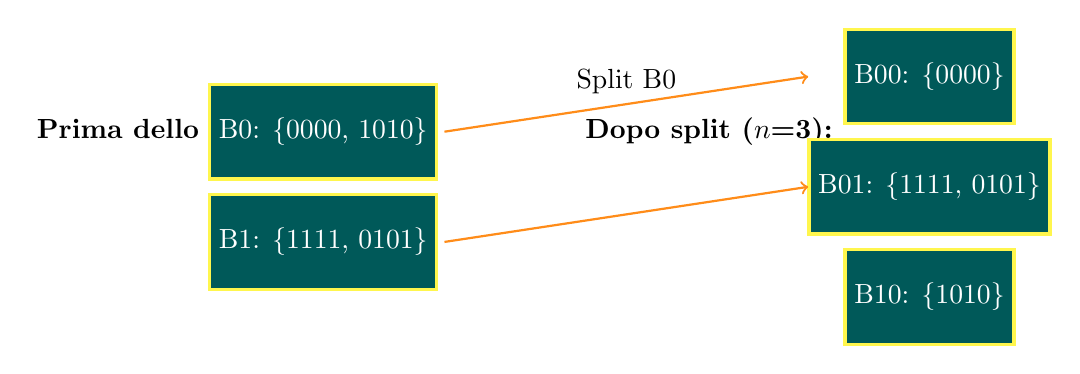
\begin{tikzpicture}[scale=0.7]
    % Stili
    \tikzset{
        bucket/.style={rectangle, draw, fill=teal!70!black, text=white, minimum width=2cm, minimum height=1.2cm, line width=1.2pt, draw=yellow!70, text centered},
        arrow/.style={->, thick, draw=orange!90}
    }
    
    % Stato iniziale (2 bucket)
    \node at (-3,0) {\textbf{Prima dello split:}};
    \node[bucket] (b0) at (0,0) {B0: \{0000, 1010\}};
    \node[bucket] (b1) at (0,-2) {B1: \{1111, 0101\}};
    
    % Stato dopo split (3 bucket)
    \node at (7,0) {\textbf{Dopo split ($n$=3):}};
    \node[bucket] (b00) at (11,1) {B00: \{0000\}};
    \node[bucket] (b01) at (11,-1) {B01: \{1111, 0101\}};
    \node[bucket] (b10) at (11,-3) {B10: \{1010\}};
    
    % Frecce
    \draw[arrow] (2.2,0) -- node[above] {Split B0} (8.8,1);
    \draw[arrow] (2.2,-2) -- node[above] {} (8.8,-1);
\end{tikzpicture}
\caption{Visualizzazione dello split nell'hashing lineare}
\end{figure}

\begin{center}
\begin{tabular}{|c|c|}
\hline
\textbf{Domanda} & \textbf{Risposta} \\
\hline
Quanti bucket? & 3 (dopo split) \\
\hline
Quanti blocchi? & 3 (ogni bucket ha un blocco) \\
\hline
\end{tabular}
\end{center}

\paragraph{Tabella Riassuntiva di Confronto}
\begin{table}[h]
\centering
\begin{tabular}{|p{3cm}|p{3.5cm}|p{3.5cm}|p{3.5cm}|}
\hline
\textbf{Caratteristica} & \textbf{Hashing Statico} & \textbf{Hashing Estensibile} & \textbf{Hashing Lineare} \\
\hline
Crescita & Nessuna (fisso) & A potenze di 2 & Lineare (uno a uno) \\
\hline
Blocchi overflow & Sì & No & Sì \\
\hline
Funzione hash & $H_i(K)$ (primi $i$ bit) & $H_i(K)$ (primi $i$ bit) & $H_i(K)$ (ultimi $i$ bit) \\
\hline
Directory & No & Sì & No \\
\hline
Complessità ricerca & $O(1)$ senza overflow & $O(1)$ se directory in RAM & $O(1)$ (più complessa) \\
\hline
\end{tabular}
\caption{Confronto tra le tre tecniche di hashing}
\end{table}

\section{Recupero di Documenti (Document Retrieval) e Indici Invertiti}
L'Information Retrieval (IR) si occupa di trovare materiale (solitamente documenti testuali non strutturati) che soddisfi un bisogno informativo all'interno di grandi collezioni. Il recupero di documenti basato su parole chiave è un problema classico.

\subsection{Indici Invertiti (Inverted Indexes)}
Sono usati per recuperare efficientemente documenti tramite query full-text.
Due tipi di query principali:
\begin{enumerate}
    \item Trovare tutti i documenti che contengono un \textbf{dato insieme di parole chiave} (es. "Brutus" AND "Caesar"). L'ordine non conta.
    \item Trovare tutti i documenti che contengono una \textbf{data sequenza di parole chiave} (es. la frase "a clear"). L'ordine conta.
\end{enumerate}
Un indice invertito, invece di creare un indice per ogni "attributo" (parola), rappresenta per ogni parola specifica (termine) l'elenco di tutti i documenti in cui appare.

\subsection{Costruzione di un Indice Invertito}
\begin{enumerate}
    \item \textbf{Tokenizzazione:} Dividi ogni documento in parole (token). Registra la posizione di ogni token.
    \begin{itemize}
        \item D1: "Friends, Romans, countrymen, lend(4) me your ears; I come to(10) bury Caesar(12), not to(14) praise him..." (numeri sono posizioni indicative)
        \item D2: "In a(2) broad valley(4), at the foot of a(9) sloping hillside, beside a(13) clear(14) bubbling stream, Tom(17) was building..."
        \item D3: "I(1) did enact Julius Caesar(5): I(6) was killed i' the Capitol; Brutus(12) killed me. It was a brute part of him(21) to kill so capital a..."
    \end{itemize}
    \item \textbf{Creazione del Dizionario (Vocabulary) e delle Posting List:}
    Il dizionario contiene tutti i termini unici. Per ogni termine, la posting list memorizza \texttt{(DocumentID, posizione)} o \texttt{(DocumentID, [lista\_posizioni])}.
\end{enumerate}

\textbf{Esempio di Indice Invertito risultante:}
\begin{itemize}
    \item \texttt{a}: (D2,2), (D2,9), (D2,13)
    \item \texttt{Brutus}: (D3,12)
    \item \texttt{Caesar}: (D1,12), (D3,5)
    \item \texttt{clear}: (D2,14)
    \item \texttt{him}: (D3,21)
    \item \texttt{I}: (D3,1), (D3,6)
    \item \texttt{lend}: (D1,4)
    \item \texttt{valley}: (D2,4)
    \item \dots (e così via per tutti i termini)
\end{itemize}

\subsection{Preprocessing Linguistico}
Per migliorare velocità e accuratezza:
\begin{itemize}
    \item \textbf{Normalizzazione dei Token:} Uniformare le parole. Es. "Windows" $\rightarrow$ "windows" (case folding). "U.S.A." $\rightarrow$ "USA".
    \item \textbf{Stemming (Radicazione):} Ricondurre le parole alla loro radice (stem). Es. "fishing", "fished", "fisher" $\rightarrow$ "fish". Aiuta a trovare documenti rilevanti anche se usano forme diverse della stessa parola.
    \item \textbf{Stop Words:} Rimuovere parole comuni (articoli, preposizioni come "the", "a", "is", "and") perché appaiono in troppi documenti e non sono discriminanti, oltre a ridurre la dimensione dell'indice.
\end{itemize}

\subsection{Esecuzione di Query con Indici Invertiti}

\textbf{Query di Insieme (Set Query - es. AND)}
"Trova documenti che contengono SIA 'Brutus' CHE 'Caesar'."
\begin{enumerate}
    \item Prendi la posting list (solo DocID) per "Brutus": \{D3\}.
    \item Prendi la posting list (solo DocID) per "Caesar": \{D1, D3\}.
    \item Interseca le liste di DocID: \{D3\} $\cap$ \{D1, D3\} = \{D3\}.
\end{enumerate}
Risultato: Documento D3.

\textbf{Query di Sequenza (Phrase Query)}
"Trova documenti che contengono la sequenza 'a valley'."
\begin{enumerate}
    \item Posting list per "a": $L_a = [(\text{D2},2), (\text{D2},9), (\text{D2},13)]$
    \item Posting list per "valley": $L_v = [(\text{D2},4)]$
    \item Per ogni $(doc\_id1, pos1)$ in $L_a$ e ogni $(doc\_id2, pos2)$ in $L_v$:
    \begin{itemize}
        \item Se $doc\_id1 == doc\_id2$ E $pos2 == pos1 + 1$, allora la sequenza è trovata.
    \end{itemize}
    \item Confronto:
    \begin{itemize}
        \item Per "a": $(\text{D2},2)$. Per "valley": $(\text{D2},4)$. DocID uguali (D2). Posizione di "valley" (4) è uguale a posizione di "a" (2) + 1? No ($4 \ne 3$).
        \item ... (altri confronti non producono match)
    \end{itemize}
\end{enumerate}
Risultato: Nessun documento contiene la sequenza "a valley".

"Trova documenti che contengono la sequenza 'a clear'."
\begin{enumerate}
    \item Posting list per "a": $L_a = [(\text{D2},2), (\text{D2},9), (\text{D2},13)]$
    \item Posting list per "clear": $L_c = [(\text{D2},14)]$
    \item Confronto:
    \begin{itemize}
        \item Per "a": $(\text{D2},13)$. Per "clear": $(\text{D2},14)$. DocID D2. $14 == 13+1$? Sì!
    \end{itemize}
\end{enumerate}
Risultato: Documento D2 contiene la sequenza "a clear" (dove "a" è in pos 13 e "clear" in pos 14).\section{Strategie per affrontare gli esercizi}
\begin{itemize}
    \item \textbf{Hashing:}
    \begin{itemize}
        \item Identifica chiaramente il tipo di hashing (statico, estensibile, lineare).
        \item Tieni traccia dei parametri chiave ($i$, $j$ per estensibile; $i$, $n_{buck}$, $r$, soglia, split pointer $s$ per lineare).
        \item Per le inserzioni, segui meticolosamente i passi, specialmente quando avvengono split (di blocco o di directory/bucket). Disegnare la struttura aiuta molto.
        \item Quando conti bucket/blocchi, ricorda la definizione: i bucket nell'hashing estensibile sono le entry della directory, i blocchi sono le strutture dati fisiche. Nell'hashing lineare, i bucket sono $n_{buck}$, i blocchi includono quelli di overflow.
    \end{itemize}
    \item \textbf{Indici Invertiti:}
    \begin{itemize}
        \item Per la costruzione, sii preciso nel tracciare le posizioni.
        \item Per le query AND, si tratta di intersecare le liste di documenti.
        \item Per le query di sequenza, dopo aver trovato i documenti comuni, devi verificare le condizioni sulle posizioni.
    \end{itemize}
\end{itemize}

